\subsection{Quasi-independence and structural zeros}\label{sec:ca-quasi}
\ixon{quasi-independence}
\ixon{structural zeros}
\ixon{zeros!structural}
Incomplete tables can result when particular cells are simply not observed
(sampling zeros, e.g., insufficient data collected) or when some combinations of levels cannot logically occur (structural zeros, e.g., pregnant males).
Alternatively, in some cases we may wish to ignore the data in some cells,
and fit a quasi-independence model to the remaining cells. This is commonly
done with square tables having the same row and column categories,
where the dominant diagonal cells cause a global independence model to fail.

Because CA decomposes departures from independence,
many of these cases can be handled simply by estimating the expected
frequencies which would occur in these cells
if the row and column variables were
independent, and replacing the zero, missing, or dominant observed
frequencies by their expected values.%
\footnote{This does not, however, account properly for the loss in
degrees of freedom, but significance tests in CA are usually not
treated formally.
Indeed, the method would be of little interest for data in which
independence holds.}
More general, iterative procedures are discussed by \citet[\S 8.5]{Greenacre:84}
and by \citet[Ch. 3]{Heijden:87}.

\begin{Example}[victims3]{Repeat victimization}
\exref{ex:victims} also showed a mosaic display 
(\figref{fig:victims3}) for the model of quasi-independence
ignoring the diagonal cells in the repeat victimization data.
The analysis below gives another view of this model.

The elements in the diagonal cells of the \pname{VICTIMS} \Dset\
can be replaced by their expected frequencies under independence
in the following \IML\ step.
\begin{listing}
proc iml;
   use victims;
   read all var _num_  into table[r=crime c=vars];
   read all var {crime} into crime;
   close victims;

   exp = table[,+] * table[+,] / table[+,+];
   table = table + diag(vecdiag(exp - table));

   create victims from table[r=crime c=vars];
   append from table[r=crime c=vars];
\end{listing}
Using the same \verb|%CORRESP| step and plotting steps
as in \exref{ex:victims2} (with a different \stmt{LEGEND}{GPLOT})
gives the 2D plot shown in
\figref{fig:corresp5b}.

%% one figure
\begin{figure}[htb]
  \centering
  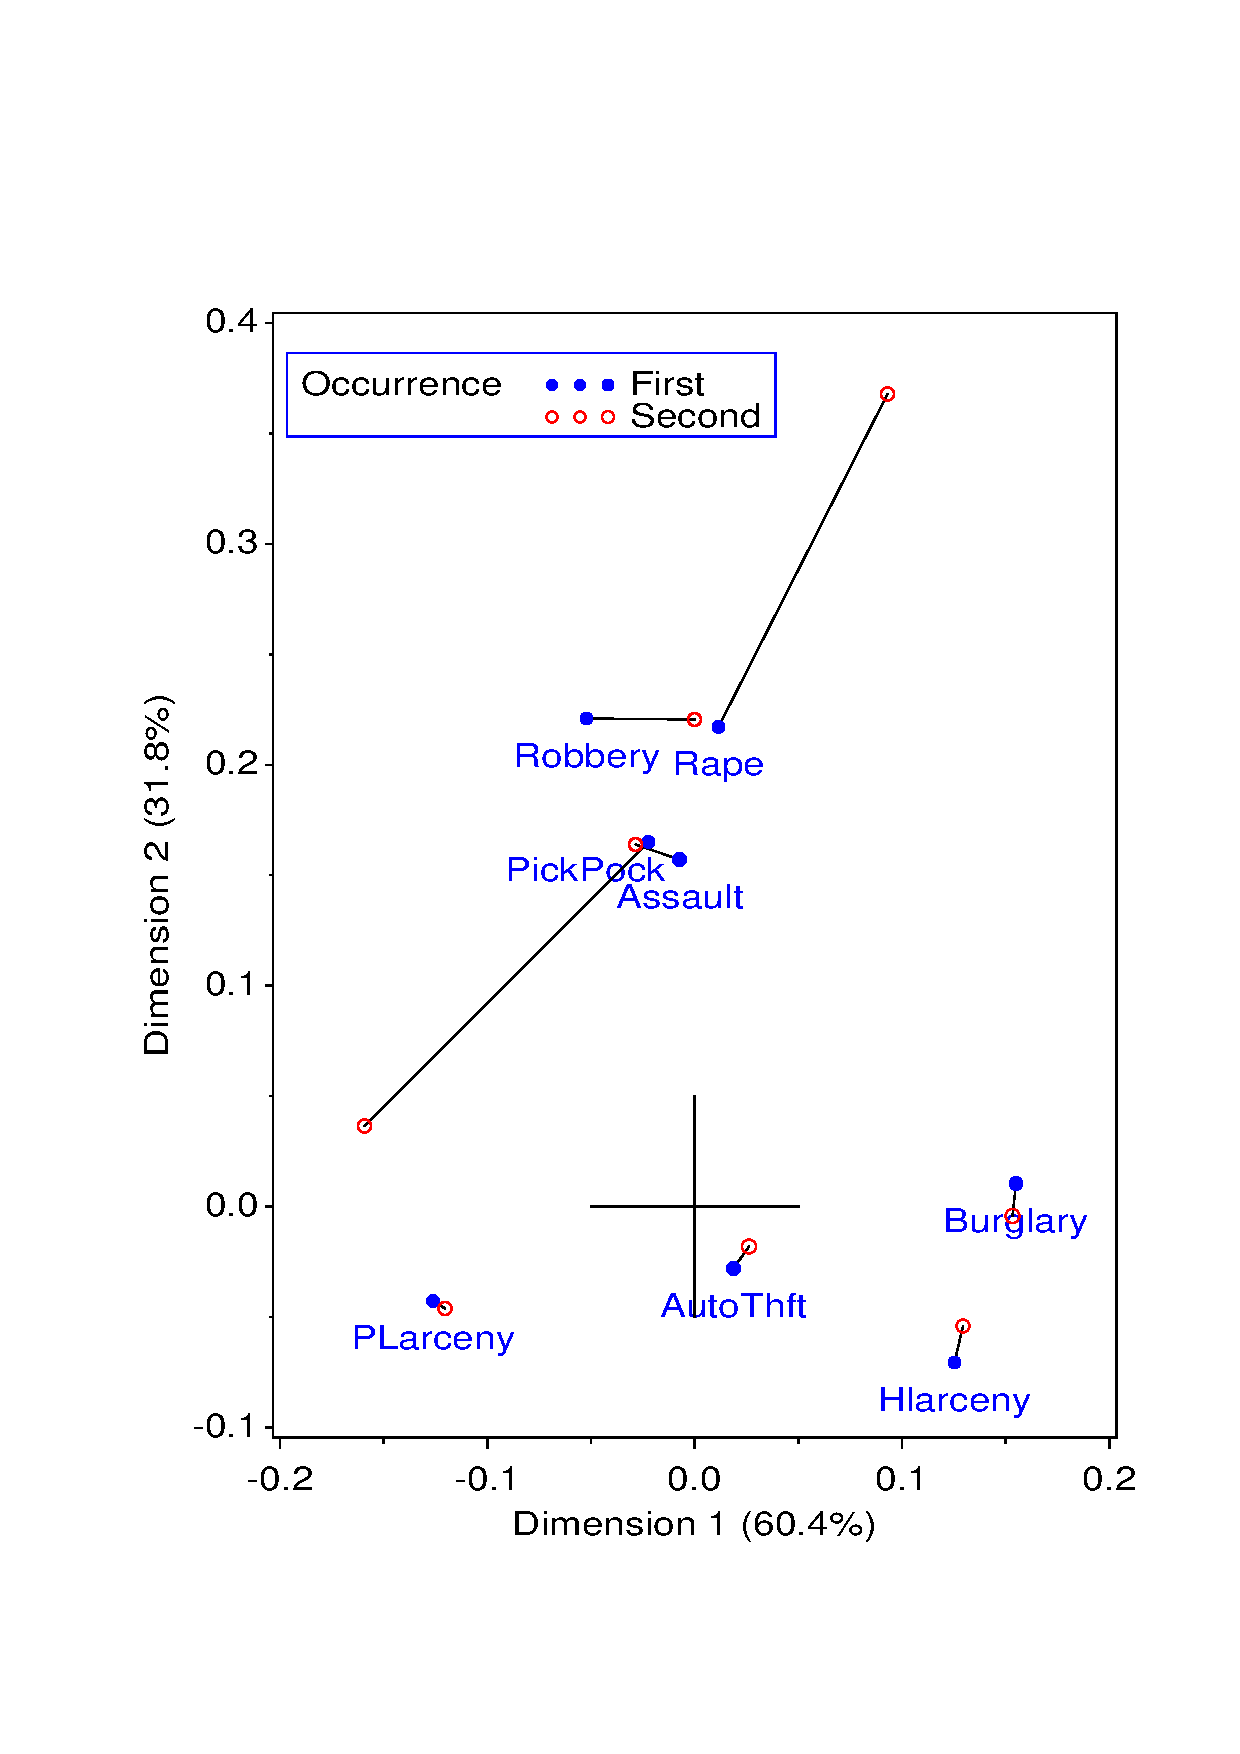
\includegraphics[scale=.6,clip]{ch5/fig/corresp5b}
  \caption[Repeat victimization data, quasi-independence
  model]{2D \CA\ display for repeat victimization data, quasi-independence
  model, ignoring diagonal cells.}%
  \label{fig:corresp5b}
\end{figure}
Note that the 2D solution now accounts for 92\% of the remaining
association, which now concerns only the cells where the crime differs
from first to second occurrence.
For these cells, the differences between first and second incident are
magnified.
\end{Example}
\ixoff{zeros!structural}
\ixoff{structural zeros}
\ixoff{quasi-independence}
